\documentclass[twoside]{book}

% Packages required by doxygen
\usepackage{fixltx2e}
\usepackage{calc}
\usepackage{doxygen}
\usepackage[export]{adjustbox} % also loads graphicx
\usepackage{graphicx}
\usepackage[utf8]{inputenc}
\usepackage{makeidx}
\usepackage{multicol}
\usepackage{multirow}
\PassOptionsToPackage{warn}{textcomp}
\usepackage{textcomp}
\usepackage[nointegrals]{wasysym}
\usepackage[table]{xcolor}

% Font selection
\usepackage[T1]{fontenc}
\usepackage[scaled=.90]{helvet}
\usepackage{courier}
\usepackage{amssymb}
\usepackage{sectsty}
\renewcommand{\familydefault}{\sfdefault}
\allsectionsfont{%
  \fontseries{bc}\selectfont%
  \color{darkgray}%
}
\renewcommand{\DoxyLabelFont}{%
  \fontseries{bc}\selectfont%
  \color{darkgray}%
}
\newcommand{\+}{\discretionary{\mbox{\scriptsize$\hookleftarrow$}}{}{}}

% Page & text layout
\usepackage{geometry}
\geometry{%
  a4paper,%
  top=2.5cm,%
  bottom=2.5cm,%
  left=2.5cm,%
  right=2.5cm%
}
\tolerance=750
\hfuzz=15pt
\hbadness=750
\setlength{\emergencystretch}{15pt}
\setlength{\parindent}{0cm}
\setlength{\parskip}{3ex plus 2ex minus 2ex}
\makeatletter
\renewcommand{\paragraph}{%
  \@startsection{paragraph}{4}{0ex}{-1.0ex}{1.0ex}{%
    \normalfont\normalsize\bfseries\SS@parafont%
  }%
}
\renewcommand{\subparagraph}{%
  \@startsection{subparagraph}{5}{0ex}{-1.0ex}{1.0ex}{%
    \normalfont\normalsize\bfseries\SS@subparafont%
  }%
}
\makeatother

% Headers & footers
\usepackage{fancyhdr}
\pagestyle{fancyplain}
\fancyhead[LE]{\fancyplain{}{\bfseries\thepage}}
\fancyhead[CE]{\fancyplain{}{}}
\fancyhead[RE]{\fancyplain{}{\bfseries\leftmark}}
\fancyhead[LO]{\fancyplain{}{\bfseries\rightmark}}
\fancyhead[CO]{\fancyplain{}{}}
\fancyhead[RO]{\fancyplain{}{\bfseries\thepage}}
\fancyfoot[LE]{\fancyplain{}{}}
\fancyfoot[CE]{\fancyplain{}{}}
\fancyfoot[RE]{\fancyplain{}{\bfseries\scriptsize Generated by Doxygen }}
\fancyfoot[LO]{\fancyplain{}{\bfseries\scriptsize Generated by Doxygen }}
\fancyfoot[CO]{\fancyplain{}{}}
\fancyfoot[RO]{\fancyplain{}{}}
\renewcommand{\footrulewidth}{0.4pt}
\renewcommand{\chaptermark}[1]{%
  \markboth{#1}{}%
}
\renewcommand{\sectionmark}[1]{%
  \markright{\thesection\ #1}%
}

% Indices & bibliography
\usepackage{natbib}
\usepackage[titles]{tocloft}
\setcounter{tocdepth}{3}
\setcounter{secnumdepth}{5}
\makeindex

% Hyperlinks (required, but should be loaded last)
\usepackage{ifpdf}
\ifpdf
  \usepackage[pdftex,pagebackref=true]{hyperref}
\else
  \usepackage[ps2pdf,pagebackref=true]{hyperref}
\fi
\hypersetup{%
  colorlinks=true,%
  linkcolor=blue,%
  citecolor=blue,%
  unicode%
}

% Custom commands
\newcommand{\clearemptydoublepage}{%
  \newpage{\pagestyle{empty}\cleardoublepage}%
}

\usepackage{caption}
\captionsetup{labelsep=space,justification=centering,font={bf},singlelinecheck=off,skip=4pt,position=top}

%===== C O N T E N T S =====

\begin{document}

% Titlepage & ToC
\hypersetup{pageanchor=false,
             bookmarksnumbered=true,
             pdfencoding=unicode
            }
\pagenumbering{roman}
\begin{titlepage}
\vspace*{7cm}
\begin{center}%
{\Large My Project }\\
\vspace*{1cm}
{\large Generated by Doxygen 1.8.11}\\
\end{center}
\end{titlepage}
\clearemptydoublepage
\tableofcontents
\clearemptydoublepage
\pagenumbering{arabic}
\hypersetup{pageanchor=true}

%--- Begin generated contents ---
\chapter{Class Index}
\section{Class List}
Here are the classes, structs, unions and interfaces with brief descriptions\+:\begin{DoxyCompactList}
\item\contentsline{section}{\hyperlink{structEEP__strings}{E\+E\+P\+\_\+strings} }{\pageref{structEEP__strings}}{}
\item\contentsline{section}{\hyperlink{structstates}{states} }{\pageref{structstates}}{}
\end{DoxyCompactList}

\chapter{Class Documentation}
\hypertarget{structEEP__strings}{}\section{E\+E\+P\+\_\+strings Struct Reference}
\label{structEEP__strings}\index{E\+E\+P\+\_\+strings@{E\+E\+P\+\_\+strings}}
\subsection*{Public Attributes}
\begin{DoxyCompactItemize}
\item 
char \hyperlink{structEEP__strings_a306b42bbc00f8f0fad740a488b716b58}{Network\+\_\+\+S\+S\+ID} \mbox{[}32\mbox{]}
\begin{DoxyCompactList}\small\item\em $<$ Strings which have stored in eeprom \end{DoxyCompactList}\item 
char \hyperlink{structEEP__strings_a6244224cc32d54c75024d6f45ead702b}{Network\+\_\+password} \mbox{[}32\mbox{]}\hypertarget{structEEP__strings_a6244224cc32d54c75024d6f45ead702b}{}\label{structEEP__strings_a6244224cc32d54c75024d6f45ead702b}

\begin{DoxyCompactList}\small\item\em password of that network \end{DoxyCompactList}\end{DoxyCompactItemize}


\subsection{Member Data Documentation}
\index{E\+E\+P\+\_\+strings@{E\+E\+P\+\_\+strings}!Network\+\_\+\+S\+S\+ID@{Network\+\_\+\+S\+S\+ID}}
\index{Network\+\_\+\+S\+S\+ID@{Network\+\_\+\+S\+S\+ID}!E\+E\+P\+\_\+strings@{E\+E\+P\+\_\+strings}}
\subsubsection[{\texorpdfstring{Network\+\_\+\+S\+S\+ID}{Network_SSID}}]{\setlength{\rightskip}{0pt plus 5cm}char E\+E\+P\+\_\+strings\+::\+Network\+\_\+\+S\+S\+ID\mbox{[}32\mbox{]}}\hypertarget{structEEP__strings_a306b42bbc00f8f0fad740a488b716b58}{}\label{structEEP__strings_a306b42bbc00f8f0fad740a488b716b58}


$<$ Strings which have stored in eeprom 

Name of S\+S\+ID to connect 

The documentation for this struct was generated from the following file\+:\begin{DoxyCompactItemize}
\item 
E\+S\+P.\+cpp\end{DoxyCompactItemize}

\hypertarget{structstates}{}\section{states Struct Reference}
\label{structstates}\index{states@{states}}


Collaboration diagram for states\+:
\nopagebreak
\begin{figure}[H]
\begin{center}
\leavevmode
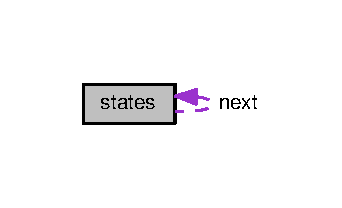
\includegraphics[width=164pt]{structstates__coll__graph}
\end{center}
\end{figure}
\subsection*{Public Attributes}
\begin{DoxyCompactItemize}
\item 
struct \hyperlink{structstates}{states} $\ast$ \hyperlink{structstates_ae75c03bfd8b1791f7e87b217dbe8d33e}{next}
\begin{DoxyCompactList}\small\item\em $<$ State Variable \end{DoxyCompactList}\item 
int($\ast$ \hyperlink{structstates_a647021e88880a0c475530c45589917f2}{state\+Func} )()\hypertarget{structstates_a647021e88880a0c475530c45589917f2}{}\label{structstates_a647021e88880a0c475530c45589917f2}

\begin{DoxyCompactList}\small\item\em State function pointer for hooking up the function. \end{DoxyCompactList}\end{DoxyCompactItemize}


\subsection{Member Data Documentation}
\index{states@{states}!next@{next}}
\index{next@{next}!states@{states}}
\subsubsection[{\texorpdfstring{next}{next}}]{\setlength{\rightskip}{0pt plus 5cm}struct {\bf states}$\ast$ states\+::next}\hypertarget{structstates_ae75c03bfd8b1791f7e87b217dbe8d33e}{}\label{structstates_ae75c03bfd8b1791f7e87b217dbe8d33e}


$<$ State Variable 

State Variable pointer for holding the next state, Link list 

The documentation for this struct was generated from the following file\+:\begin{DoxyCompactItemize}
\item 
E\+S\+P.\+cpp\end{DoxyCompactItemize}

%--- End generated contents ---

% Index
\backmatter
\newpage
\phantomsection
\clearemptydoublepage
\addcontentsline{toc}{chapter}{Index}
\printindex

\end{document}
